\begin{figure}[!htbp]
\centering
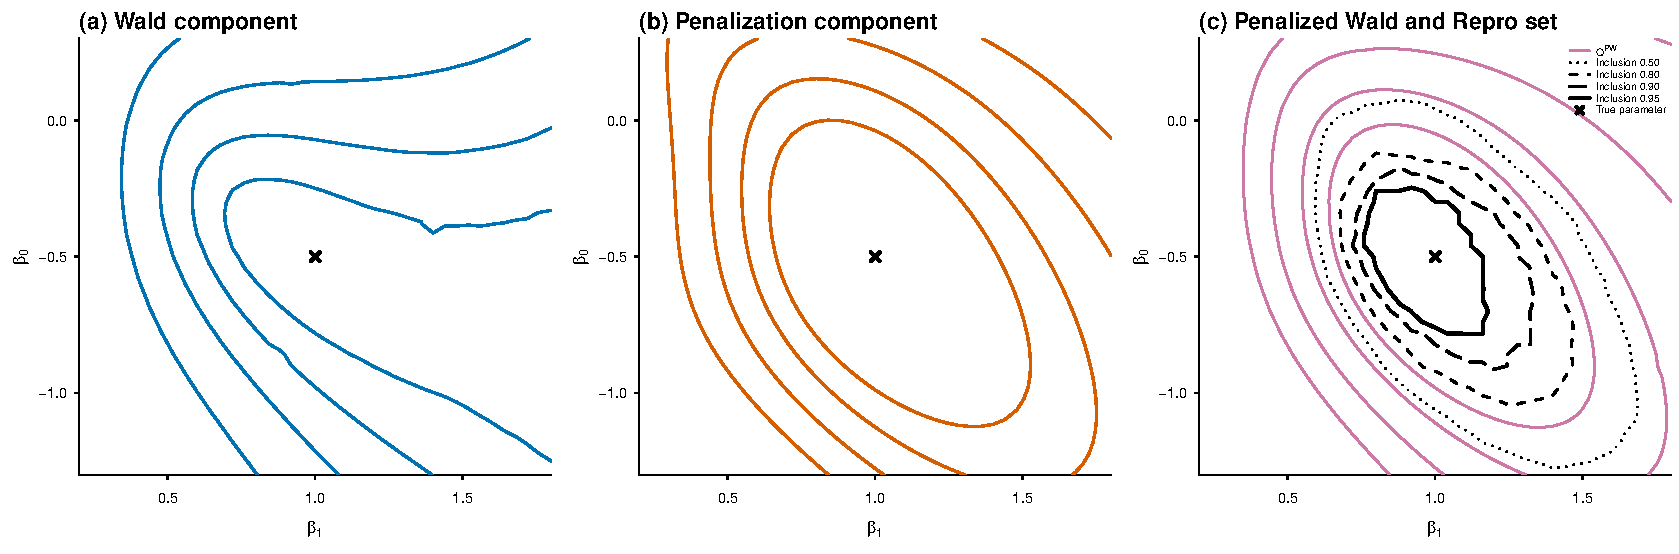
\includegraphics[width=0.92\linewidth]{results/figures/fig_exp2_sigma_geometry.pdf}
\caption{Experiment 2, $\sigma$ target. Monte Carlo mean level sets in the $(\beta_1,\beta_0)$ nuisance section, with the remaining coordinates fixed at their true values: the nuisance-orthogonal Wald component, the Mahalanobis penalty, and the combined statistic. The figure carries information the summary table does not, namely the shape of the accepted set in the nuisance directions and the relative contribution of the two components.}
\label{fig:exp2-sigma-geometry}
\end{figure}
